\documentclass[
  jou,
  colorlinks=true,linkcolor=blue,citecolor=blue,urlcolor=blue]{apa7}

% TODO: Add custom LaTeX header directives here
\makeatletter
\renewcommand{\paragraph}{\@startsection{paragraph}{4}{\parindent}%
	{0\baselineskip \@plus 0.2ex \@minus 0.2ex}%
	{-.5em}%
	{\normalfont\normalsize\bfseries\typesectitle}}

\renewcommand{\subparagraph}[1]{\@startsection{subparagraph}{5}{0.5em}%
	{0\baselineskip \@plus 0.2ex \@minus 0.2ex}%
	{-\z@\relax}%
	{\normalfont\normalsize\bfseries\itshape\hspace{\parindent}{#1}\textit{\addperi}}{\relax}}
\makeatother

\usepackage{fontspec}
\usepackage{multirow}
\usepackage{multicol}
\usepackage{colortbl}
\usepackage{hhline}
\newlength\Oldarrayrulewidth
\newlength\Oldtabcolsep
\usepackage{longtable}
\usepackage{array}
\usepackage{hyperref}
\usepackage{float}
\usepackage{wrapfig}\makeatletter\makeatother\makeatletter\makeatother\makeatletter\@ifpackageloaded{caption}{}{\usepackage{caption}}\AtBeginDocument{%
\ifdefined\contentsname
  \renewcommand*\contentsname{Table of contents}
\else
  \newcommand\contentsname{Table of contents}
\fi
\ifdefined\listfigurename
  \renewcommand*\listfigurename{List of Figures}
\else
  \newcommand\listfigurename{List of Figures}
\fi
\ifdefined\listtablename
  \renewcommand*\listtablename{List of Tables}
\else
  \newcommand\listtablename{List of Tables}
\fi
\ifdefined\figurename
  \renewcommand*\figurename{Figure}
\else
  \newcommand\figurename{Figure}
\fi
\ifdefined\tablename
  \renewcommand*\tablename{Table}
\else
  \newcommand\tablename{Table}
\fi
}\@ifpackageloaded{float}{}{\usepackage{float}}
\floatstyle{ruled}
\@ifundefined{c@chapter}{\newfloat{codelisting}{h}{lop}}{\newfloat{codelisting}{h}{lop}[chapter]}
\floatname{codelisting}{Listing}\newcommand*\listoflistings{\listof{codelisting}{List of Listings}}\makeatother\makeatletter\@ifpackageloaded{caption}{}{\usepackage{caption}}
\@ifpackageloaded{subcaption}{}{\usepackage{subcaption}}\makeatother\makeatletter\@ifpackageloaded{tcolorbox}{}{\usepackage[skins,breakable]{tcolorbox}}\makeatother\makeatletter\@ifundefined{shadecolor}{\definecolor{shadecolor}{rgb}{.97, .97, .97}}\makeatother\makeatletter\makeatother\makeatletter\makeatother



% \usepackage[style=apa,backend=biber]{biblatex}
% % \addbibresource{bibliography.bib}
% 
\newlength{\cslhangindent}
\setlength{\cslhangindent}{1.5em}
\newlength{\csllabelwidth}
\setlength{\csllabelwidth}{3em}
\newlength{\cslentryspacingunit} % times entry-spacing
\setlength{\cslentryspacingunit}{\parskip}
\newenvironment{CSLReferences}[2] % #1 hanging-ident, #2 entry spacing
 {% don't indent paragraphs
  \setlength{\parindent}{0pt}
  % turn on hanging indent if param 1 is 1
  \ifodd #1
  \let\oldpar\par
  \def\par{\hangindent=\cslhangindent\oldpar}
  \fi
  % set entry spacing
  \setlength{\parskip}{#2\cslentryspacingunit}
 }%
 {}
\usepackage{calc}
\newcommand{\CSLBlock}[1]{#1\hfill\break}
\newcommand{\CSLLeftMargin}[1]{\parbox[t]{\csllabelwidth}{#1}}
\newcommand{\CSLRightInline}[1]{\parbox[t]{\linewidth - \csllabelwidth}{#1}\break}
\newcommand{\CSLIndent}[1]{\hspace{\cslhangindent}#1}

\title{The Relationship Between Fundamental Movement Skills and Body
Mass Index in Elementary-Age Children}
\shorttitle{Template for the APAquarto Format}




\authorsnames[{1},{2}]{
Mariah Bolin,Ovande Furtado Jr
}

\authorsaffiliations{
{Seneca High School},{Department of Kinesiology, California State
University, Northridge}}

\date{}
\abstract{Mastery of fundamental movement skills (FMS) is considered a
crucial component in securing physical activity participation and, in
turn, decreasing the likelihood of obesity. This study aimed to
investigate the relationship between body mass index (BMI) and FMS
performance among children ages 5 to 7 years in a rural school system.
Secondly, we intended to investigate BMI grouping and gender differences
in FMS performance. Participants were 39 kindergarteners and 1st graders
(20 boys and 19 girls) in an Eastern Illinois K--8 public school. BMI
was calculated for each participant using CDC guidelines (CDC, 2008).
FMS performance was assessed using the Furtado-Gallagher Computerized
Observational Movement Pattern Assessment System (FG-COMPASS). Pearson
correlation coefficients were calculated to examine the relationship
between BMI percentile and FMS performance. A small but negative
correlation that was not significant was found for FMS Locomotor, r(2) =
-- .26, p \textgreater{} 05, and FMS Total r(2) = - .20, p
\textgreater{} 05. In addition, a Two-way Factorial MANOVA was conducted
to determine the effect of BMI levels and gender on the performance of
FMS. MANOVA results indicated that gender, Wilks' Lamda = .637, F(2,32)
= 11.23, p \textless{} .001, significantly affected the combined
dependent variables. No significant main effect was detected for BMI
levels. Univariate analysis of variance post-hoc tests revealed that the
performance of manipulative FMS significantly differs for gender,
F(1,33) = 16.08, p \textless{} .001, with males (M = 12.38, SD = 2.8)
overperforming females (M = 9.11, SD = 2.21). Performance of locomotor
fundamental movement skills does not significantly differ for gender.
These findings have implications for educators and health professionals
working with rural children. Programs must ensure that boys and girls
have equal opportunities to practice and master manipulative FMS.}
% % \addbibresource{bibliography.bib}
% 
\keywords{body mass index, fundamental movement
skills, obesity, physical activity}

\authornote{\par{\addORCIDlink{Mariah
Bolin}{0009-0008-9190-4238}}\par{\addORCIDlink{Ovande Furtado
Jr}{0000-0003-3847-6314}}
\par{ }
\par{        }
\par{Correspondence concerning this article should be addressed to Ovande
Furtado Jr, Department of Kinesiology, California State University,
Northridge, 18111 Nordhoff St, Northridge, CA 91330-8287}}


\begin{document}
\maketitle
\ifdefined\Shaded\renewenvironment{Shaded}{\begin{tcolorbox}[boxrule=0pt, interior hidden, borderline west={3pt}{0pt}{shadecolor}, enhanced, frame hidden, breakable, sharp corners]}{\end{tcolorbox}}\fi
According to the National Centers for Disease Control and Prevention
(2022), childhood obesity has almost tripled since 1980. The occurrence
of obesity in 1st-grade to 5th-grade students has increased from 6.5\%
in 1980 to 19.6\% in 2008. In grades 6\textsuperscript{th} through
12\textsuperscript{th}, the percentage has risen from 5.0\% to 18.1\%.
Obesity can be caused by several factors, including but not limited to
low-energy supply, inactivity, and possible genetic predisposition.
Children who are overweight/obese have a greater chance of remaining
overweight/obese throughout adolescence and into adulthood (Nader et
al., 2006). In addition, health conditions such as diabetes,
hypertension, and cardiovascular disease may be absent during childhood
but may appear as the individual ages (Daniels, 2006). Thus, we must
understand the relationship between obesity and other related variables,
such as fundamental movement skills - FMS (e.g., skipping, galloping,
hopping, overhand throwing, kicking, dribbling, etc.).

Evidence shows that overweight children may be less proficient in
fundamental movement skills than non-overweight children. This
relationship may be an extension of infant weight and motor activity
relationships (Wrotniak et al., 2006). In addition, overweight children
tend to engage less often in physical activities, preventing them from
acquiring fundamental movement skills (Logan et al., 2011). Therefore,
it is essential to study the relationship between children's weight and
FMS levels in young children to learn when and how this relationship
occurs (Logan et al., 2011). With this knowledge, practitioners can
better address intervention practices in school settings.

Furthermore, previous studies have shown that children who become
proficient in FMSs are more likely to be physically active and take part
in physical activity when compared to their counterparts with a lesser
level of motor skill proficiency (Wrotniak et al., 2006). In addition,
FMS proficiency is considered the basis for developing more complex
(specialized) motor skills (Barnett et al., 2008). However, the
association between motor skill proficiency and regular participation in
physical activity begins in early childhood, fully matures in the
teenage years, and continues into adulthood (Stodden et al., 2008).
Thus, children lacking fundamental movement skill development will
likely have decreased participation in activities involving skills such
as running, jumping, skipping, or specialized sport-related skills
during the middle to late childhood, which could impact an active
lifestyle as they age (Lopes et al., 2012).

It is commonly believed that fundamental movement skills solely develop
with maturation and are not significantly impacted by environmental
factors (Clark, 2007). However, while maturation does play a role in the
development of these skills, it is not the only factor at play. The
environment, chances for practice, reassurance, and teaching all
contribute to developing fundamental movement skills (Gallahue \& Ozmun,
1998). Studies have shown that there are notable gender differences in
manipulative and locomotor skills. According to Barnett et al.~(2008),
males tend to excel in executing manipulative skills like catching,
overhand throwing, and kicking when compared to females.

On the other hand, females scored slightly higher on locomotor skills,
but the difference was not statistically significant. In another study,
Wozniak et al.~(2006) found that males overperformed females on running
speed, and agility and were more successful at the skill of overhand
throw. Dissimilarities in males' and females' motor proficiency can be
attributed to environmental factors and peer interaction. According to
Wrotniak (2006), this could be due to the type of sports and games they
are drawn to participate in, which may give males more opportunities to
practice and refine motor skills. Males are drawn to more sports
involving manipulative skills than locomotor skills.

Therefore, this study aimed to investigate the relationship between body
mass index (BMI) and FMS performance among children ages 5 to 7 years in
a rural school system. In addition, we sought to investigate BMI
grouping and gender differences in FMS performance.

We hypothesized a significant correlation between BMI and FMS
performance (FMS locomotor, FMS manipulative, and FMS total). We also
predicted that males would overperform females on manipulative skills
but not on locomotor skills. Finally, we hypothesize that the
performance of manipulative and locomotor skills would differ by BMI
levels. Children categorized as ``normal weight'' would overperform
their counterparts categorized as ``overweight'' and ``obese.''

\hypertarget{method}{%
\section{Method}\label{method}}

\hypertarget{participants}{%
\subsection{Participants}\label{participants}}

Twenty boys (mean age in months = 78.8, SD=8.17) and 19 girls (mean age
in months = 79.0, SD=9.76) participated in this study. The sample came
from a K-6 public school in Shelby County, Illinois. Most students were
Caucasian (99\%), and over 50\% of the parents whose children attended
the school were considered low-income families. Because prospective
participants were required to perform various fundamental movement
skills (e.g., skipping, running, throwing) as part of the research
protocol, children with special needs were excluded from this study. A
letter briefly explaining the study's purpose, along with the informed
consent, was sent to parents. Two weeks after the initial contact, we
emailed only those parents who still need to return the signed informed
consent. Only those children whose parents signed and returned the
informed consent were selected to be part of the study. Research
procedures were approved through the Eastern Illinois University
Institutional Review Board. To encourage student participation in the
study, those who submitted their informed consent form on time were
given a pedometer as a reward.

\hypertarget{instrumentation-and-procedures}{%
\subsection{Instrumentation and
Procedures}\label{instrumentation-and-procedures}}

\hypertarget{anthropometry}{%
\subsubsection{Anthropometry}\label{anthropometry}}

Eligible students had their height and weight measured. Mass was
measured on a calibrated electronic scale (EatSmart Products Precision
Digital) to the nearest 0.1 pounds before being later converted to
kilograms. We measured students with shoes and heavy clothing removed.
The scale was calibrated using a 10-pound weight after every 15 students
were measured to ensure scale accuracy. Height was measured to the
nearest millimeter using a tape taped to the wall. Students were
barefoot and stood with their backs to the wall while their height was
being taken. Participants' height and weight measurements were used to
calculate the BMI of each student.

\hypertarget{fundamental-movement-skill-proficiency}{%
\subsubsection{Fundamental Movement Skill
Proficiency}\label{fundamental-movement-skill-proficiency}}

Like the anthropometric data, we assessed FMS proficiency during the
daily physical education classes. The gym was split in two so that
assessment and the physical education class could be carried out
concurrently. Students were taken five at a time from their physical
education classes and videotaped while performing the fundamental
movement skills per the test protocol's instructions. A trained person
administered the Furtado-Gallagher Computerized Observational Movement
Pattern Assessment System (FG-COMPASS).

The FG-COMPASS is a criterion-related and process-oriented assessment
tool developed for school settings. Content-related validity evidence
and reliability of classification decisions (Furtado \& Gallagher, 2012)
have been reported for the FG-COMPASS. We collected data on three
locomotor (hop, horizontal jump, and skip) and five manipulative (throw,
strike, kick, hand dribble, and catch) skills.

\hypertarget{scoring}{%
\subsubsection{Scoring}\label{scoring}}

BMI was calculated for each participant, and scores were converted to
percentile ranks following the CDC guidelines (CDC, 2022b). In addition,
participants were classified based on the following criteria:
underweight - less than the 5th\%; health weight - 5th\% to less than
the 85th\%; overweight - 85th\% to less than the 95th\%; and obesity -
equal or greater than the 95th\%.~~

Before FMS data collection, the principal investigator (PI) coding the
videos was trained to become familiar with the test protocol. Videos of
children performing locomotor and manipulative skills were used for
training purposes. The PI and someone highly experienced with the
FG-COMPASS testing protocol classified eight videos per skill.
Classification scores between the PI and the expert were compared, and
disagreements were discussed between the two raters. This served to
improve the internal validity of this study. Per the test's protocol,
children are coded as 1, 2, 3, or 4 based on their performance on each
fundamental movement skill. We added the scores for each skill within
their respective subscale. Each participant was assigned a score for the
locomotor subscale, the manipulative subscale, and the total test (i.e.,
subscales combined).

\hypertarget{statistical-analyses}{%
\subsection{Statistical Analyses}\label{statistical-analyses}}

The Pearson product-moment correlation was used to investigate the
relationship between BMI percentile and the FG-COMPASS scores. We
conducted three separate analyses, one for each subscale and one for the
total test. We followed Cohen's (1988) guidelines to interpret the
associations: 0.1 \textless{} \textbar{} r \textbar{} \textless{} .3
(small correlation); 0.3 \textless{} \textbar{} r \textbar{} \textless{}
.5 (medium/moderate correlation); and \textbar{} r \textbar{}
\textgreater{} .5 (large/strong correlation).

Additionally, a two-way factorial multivariate analysis of variance
(MANOVA) was conducted to determine gender and BMI level differences in
fundamental movement skill performance. Gender and BMI groups served as
the two independent variables, and the FG-COMPASS's locomotor and
manipulative subscales served as the model's two dependent variables.
The weight status categories and percentile ranges suggested by CDC
(CDC, 2008) were used to separate the participants into groups according
to BMI levels. Because only one participant fell under the
``underweight'' category, we decided to combine it with'' healthy
weight'' and name this new category ``normal weight''. This produced the
following groups: Normal Weight (less than the 85\textsuperscript{th}
percentile), Overweight (85\textsuperscript{th} to less than the
95\textsuperscript{th}percentile), and Obese (equal to or greater than
the 95\textsuperscript{th} percentile). All analyses were done with
Jamovi (The jamovi project, 2022).

Table

\begin{longtable}[]{@{}
  >{\raggedright\arraybackslash}p{(\columnwidth - 14\tabcolsep) * \real{0.2368}}
  >{\raggedright\arraybackslash}p{(\columnwidth - 14\tabcolsep) * \real{0.1974}}
  >{\raggedright\arraybackslash}p{(\columnwidth - 14\tabcolsep) * \real{0.1053}}
  >{\raggedright\arraybackslash}p{(\columnwidth - 14\tabcolsep) * \real{0.0526}}
  >{\raggedright\arraybackslash}p{(\columnwidth - 14\tabcolsep) * \real{0.0921}}
  >{\raggedright\arraybackslash}p{(\columnwidth - 14\tabcolsep) * \real{0.0789}}
  >{\raggedright\arraybackslash}p{(\columnwidth - 14\tabcolsep) * \real{0.1184}}
  >{\raggedright\arraybackslash}p{(\columnwidth - 14\tabcolsep) * \real{0.1184}}@{}}
\toprule\noalign{}
\begin{minipage}[b]{\linewidth}\raggedright
\end{minipage} & \begin{minipage}[b]{\linewidth}\raggedright
BMI Group
\end{minipage} & \begin{minipage}[b]{\linewidth}\raggedright
Sex
\end{minipage} & \begin{minipage}[b]{\linewidth}\raggedright
N
\end{minipage} & \begin{minipage}[b]{\linewidth}\raggedright
Mean
\end{minipage} & \begin{minipage}[b]{\linewidth}\raggedright
SD
\end{minipage} & \begin{minipage}[b]{\linewidth}\raggedright
Min
\end{minipage} & \begin{minipage}[b]{\linewidth}\raggedright
Max
\end{minipage} \\
\midrule\noalign{}
\endhead
\bottomrule\noalign{}
\endlastfoot
FMS Locomotor & Normal Weight & Male & 14 & 7.07 & 2.62 & 3 & 11 \\
& & Female & 11 & 7.73 & 2.05 & 5 & 11 \\
& Overweight & Male & 3 & 6 & 2 & 4 & 8 \\
& & Female & 4 & 6.25 & 2.87 & 3 & 10 \\
& Obese & Male & 3 & 6 & 1.73 & 4 & 7 \\
& & Female & 4 & 8.25 & 1.5 & 6 & 9 \\
FMS Manipulative & Normal Weight & Male & 14 & 12.14 & 2.32 & 9 & 16 \\
& & Female & 11 & 9.09 & 2.26 & 6 & 12 \\
& Overweight & Male & 3 & 11.67 & 3.79 & 9 & 16 \\
& & Female & 4 & 8.75 & 0.96 & 8 & 10 \\
& Obese & Male & 3 & 13.33 & 2.31 & 12 & 16 \\
& & Female & 4 & 9.5 & 3.42 & 5 & 13 \\
\end{longtable}

\hypertarget{method-1}{%
\section{Method}\label{method-1}}

General remarks on method. This paragraph is optional.

Not all papers require each of these sections. Edit them as needed.
Consult the \href{https://apastyle.apa.org/jars}{Journal Article
Reporting Standards} for what is needed for your type of article.

\hypertarget{participants-1}{%
\subsection{Participants}\label{participants-1}}

Who are they? How were they recruited? Report criteria for participant
inclusion and exclusion. Perhaps some basic demographic stats are in
order. A table is a great way to avoid repetition in statistical
reporting.

\hypertarget{measures}{%
\subsection{Measures}\label{measures}}

This section can also be titled \textbf{Materials} or
\textbf{Apparatus}. Whatever tools, equipment, or measurement devices
used in the study should be described.

\hypertarget{measure-a}{%
\subsubsection{Measure A}\label{measure-a}}

Describe Measure A.

\hypertarget{measure-b}{%
\subsubsection{Measure B}\label{measure-b}}

Describe Measure B.

\hypertarget{procedure}{%
\subsection{Procedure}\label{procedure}}

What did participants do?

How are the data going to be analyzed?

\hypertarget{results}{%
\section{Results}\label{results}}

\hypertarget{descriptive-statistics}{%
\subsection{Descriptive Statistics}\label{descriptive-statistics}}

Here we describe the basic characteristics of our primary variables.

Let's make a figure. A reference label for a figure in APA format must
have the prefix \texttt{apafg-}. This is different from the usual Quarto
prefix \texttt{fig-}.

\begin{figure}[h!]
\caption{This is the figure caption.}
\label{apafg-myplot}
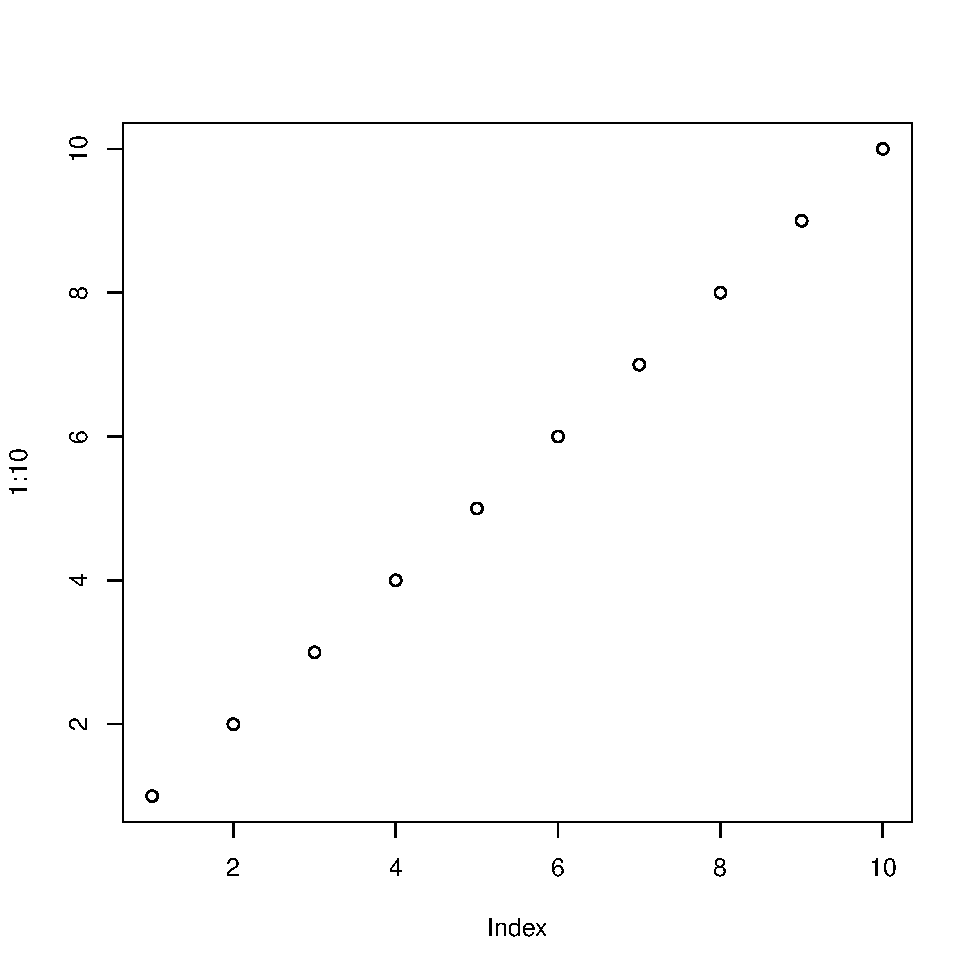
\includegraphics[width=6.5 in]{bolin23_files/figure-pdf/apafg-myplot-1.pdf}


\figurenote{This is a note below the figure.}


\end{figure}

To refer to any figure or table, put the chunk label in curly braces.
For example, see Figure~\ref{apafg-myplot}. In
Figure~\ref{apafg-importedgraphic}, we import an image.

\begin{figure}[h!]
\caption{This is an imported graphic.}
\label{apafg-importedgraphic}

\includegraphics[width=0.85in]{orcid.png}


\figurenote{My note.}


\end{figure}

We can make a table the same way as a figure except that the label
prefix is \texttt{apatb-}. Again, this is different from the usual
quarto prefix \texttt{tbl-}, which will put the table table caption in
the wrong place and with non-APA formatting.

\begin{table}
\caption{Here is the table caption.}
\label{apatb-mytable}

\global\setlength{\Oldarrayrulewidth}{\arrayrulewidth}

\global\setlength{\Oldtabcolsep}{\tabcolsep}

\setlength{\tabcolsep}{0pt}

\renewcommand*{\arraystretch}{1.5}



\providecommand{\ascline}[3]{\noalign{\global\arrayrulewidth #1}\arrayrulecolor[HTML]{#2}\cline{#3}}

\begin{longtable*}[l]{|p{0.75in}|p{0.75in}}



\ascline{0.75pt}{000000}{1-2}

\multicolumn{1}{>{\centering}m{\dimexpr 0.75in+0\tabcolsep}}{\textcolor[HTML]{000000}{\fontsize{11}{11}\selectfont{Numbers}}} & \multicolumn{1}{>{\centering}m{\dimexpr 0.75in+0\tabcolsep}}{\textcolor[HTML]{000000}{\fontsize{11}{11}\selectfont{Letters}}} \\

\ascline{0.75pt}{000000}{1-2}\endhead



\multicolumn{1}{>{\centering}m{\dimexpr 0.75in+0\tabcolsep}}{\textcolor[HTML]{000000}{\fontsize{11}{11}\selectfont{1}}} & \multicolumn{1}{>{\centering}m{\dimexpr 0.75in+0\tabcolsep}}{\textcolor[HTML]{000000}{\fontsize{11}{11}\selectfont{A}}} \\





\multicolumn{1}{>{\centering}m{\dimexpr 0.75in+0\tabcolsep}}{\textcolor[HTML]{000000}{\fontsize{11}{11}\selectfont{2}}} & \multicolumn{1}{>{\centering}m{\dimexpr 0.75in+0\tabcolsep}}{\textcolor[HTML]{000000}{\fontsize{11}{11}\selectfont{B}}} \\





\multicolumn{1}{>{\centering}m{\dimexpr 0.75in+0\tabcolsep}}{\textcolor[HTML]{000000}{\fontsize{11}{11}\selectfont{3}}} & \multicolumn{1}{>{\centering}m{\dimexpr 0.75in+0\tabcolsep}}{\textcolor[HTML]{000000}{\fontsize{11}{11}\selectfont{C}}} \\





\multicolumn{1}{>{\centering}m{\dimexpr 0.75in+0\tabcolsep}}{\textcolor[HTML]{000000}{\fontsize{11}{11}\selectfont{4}}} & \multicolumn{1}{>{\centering}m{\dimexpr 0.75in+0\tabcolsep}}{\textcolor[HTML]{000000}{\fontsize{11}{11}\selectfont{D}}} \\

\ascline{0.75pt}{000000}{1-2}



\end{longtable*}



\arrayrulecolor[HTML]{000000}

\global\setlength{\arrayrulewidth}{\Oldarrayrulewidth}

\global\setlength{\tabcolsep}{\Oldtabcolsep}

\renewcommand*{\arraystretch}{1}

\tablenote{Here is the note below the table.}

\end{table}

To refer to this table in text, put the table's reference label in curly
braces like so: As seen in Table~\ref{apatb-mytable}, there is not much
information.

What if you want the tables and figures to be at the end of the
document? In the .pdf format, you can set the \texttt{floatsintext}
option to false. For .html and .docx documents, there is not yet an
automatic way to put tables and figures at the end. You can, of course,
just put them all at the end, in order. The reference labels will work
no matter where they are in the text.

\hypertarget{discussion}{%
\section{Discussion}\label{discussion}}

Describe results in non-statistical terms.

\hypertarget{limitations-and-future-directions}{%
\subsection{Limitations and Future
Directions}\label{limitations-and-future-directions}}

Every study has limitations. Based on this study, some additional steps
might include\ldots{}

\hypertarget{conclusion}{%
\subsection{Conclusion}\label{conclusion}}

Let's sum this up.

\hypertarget{references}{%
\section{References}\label{references}}

\hypertarget{refs}{}
\begin{CSLReferences}{1}{0}
\leavevmode\vadjust pre{\hypertarget{ref-ObesityHealthySchools2022}{}}%
\emph{Obesity - {Healthy Schools}}. (2022).
\url{https://www.cdc.gov/healthyschools/obesity/index.htm}

\end{CSLReferences}

\newpage{}

\hypertarget{appendix}{%
\section{Appendix}\label{appendix}}

If there are multiple appendices, label them with level 1 headings as
Appendix A, Appendix B, and so forth.


\end{document}
